\section{Future Work}\label{Future}

As mentioned in Sections \ref{LitRev} and \ref{Progress}, a large amount of research and development has already been conducted. Nonetheless, a number of key stages still remain. This section outlines the remaining stages and goes into some detail to describe possible methods and expected outcomes.

\subsection{Encrypted Database Entry}\label{FutureEncData}

The development of encryption per database entry is probably the most crucial stage of the project. As outlined in Section 2.1.3, the most algorithm is largely simple to implement. The encryption algorithm will use is standard AES with CBC mode. 

A key decision at this point is determining the placement encryption on client or server side. The advantage of applying encryption on server side is more computational resources, but this also means that encrypted content along with encryption key need to be sent back to the client one encryption is complete, and could become expensive when data inserted to the database is large. If encryption is applied at the client side, then the encrypted data can be written into client database without having to go through server, thus saving network bandwidth.

\subsection{Possible Studies}\label{FuturePosStudy}

A number of different numerical studies can be conducted. As mentioned in Section 2.3,
the ideal outcome of these studies is a set of data that will help assess the efficiency of auditable database design.

The most basic study would be a comparison of overhead produced by added layer of EncProvider (Section 3.1). A set of real-world workload on a contact database can be recorded through tracing database query calls on the Contact database as part of the Android operating system. These queries can then be played back on the benchmark application with and without EncProvider. A wall clock time will be recorded to study the performance overhead.

A second study that will be performed is a comparison between per-row and per-column encryption as outlined in Section 2.3.2. A set predetermined queries will be played back at random time interval with each encryption method as outlined in table.

[insert Table]

\subsection{Schedule}\label{FutureSchedule}

The Gantt chart in Figure \ref{FigGantt} outlines the schedule from now until the end of the term when the final thesis document is to be delivered.

\begin{figure}[h]
  \centering
  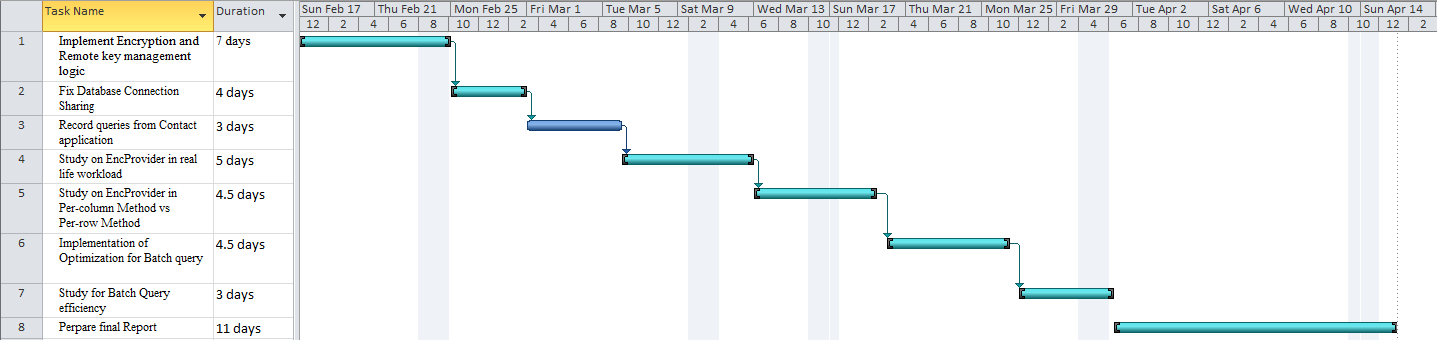
\includegraphics[scale=0.55,angle=270]{./Figs/gantt_chart.png}
  \caption[Gantt Chart of Future Work]%
  {A Gantt Chart detailing the work to be done on this project in the future.}
  \label{FigGantt}
\end{figure}
